\documentclass[../../../main.tex]{subfiles}
\begin{document}
Dispersion is the dependence of the velocity of a wave on its frequency, leading to the separation of different frequency components in a medium.
\subsection*{Beats}
Beats refer to phenomenon where waves sometimes add constructively and another times destructively because of their different frequencies. Consider superposition of two monochromatic waves
\begin{equation*}
    \psi_1=A \cos(k_1x - \omega_1t),\quad \psi_2=A \cos(k_2x - \omega_2t)
\end{equation*}
that have the same amplitude $A$ but different frequencies $\omega_1$ and $\omega_2$, respectively. In a non-dispersive medium, the two waves travel at the same velocity. The superposition of the two waves gives
\begin{align*}
    \psi(x,t)&=A\big[\cos(k_1x - \omega_1t)+ \cos(k_2x - \omega_2t)\big]\\
    \psi(x,t)&=2A\cos\bigg[\frac{k_2-k_1}{2}x-\frac{\omega_2-\omega_1}{2}t]\cos\bigg[\frac{k_2+k_1}{2}x-\frac{\omega_2+\omega_1}{2}t\bigg]
\end{align*}
We consider how $\psi$ varies at a fixed value of position $x$
\begin{equation*}
    \psi(0,t)=2A\cos\bigg[\frac{\omega_2-\omega_1}{2}t\bigg] \cos\bigg[\frac{\omega_2+\omega_1}{2}t\bigg]
\end{equation*}

The resultant wave is contained within an envelope $A(t)$ given by
\begin{equation*}
    A(t)=2A\cos\bigg[\frac{\omega_2-\omega_1}{2}t\bigg]
\end{equation*}
Thus, we can write 
\begin{equation*}
    \psi(0,t)=A(t)\cos \omega_0 t
\end{equation*}
where $\omega_0=(\omega_2+\omega_1)/2$.

\subsection*{Amplitude Modulation}
A carrier wave of frequency $\omega_c$ is modulated by a sinusoidal wave of frequency $\omega_m$, where $\omega_c \ll \omega_m$, The resultant wave can be represented by
\begin{align*}
    \psi &= (A + B \cos \omega_mt) \sin \omega_ct\\
    &=A\sin \omega_ct+\frac{B}{2}\big[\sin (\omega_c+\omega_m)t-\sin (\omega_c+\omega_m)t\big]
\end{align*}
which shows that there are three frequency components present in the modulated wave. 

\subsection*{Phase and Group Velocities}
We again consider the superposition of two monochromatic waves that have the same amplitude but slightly different frequencies. The superposition of $\psi_1$ and $\psi_2$ is the same as before 
\begin{equation*}
    \psi(x,t)=2A\cos\bigg[\frac{k_2-k_1}{2}x-\frac{\omega_2-\omega_1}{2}t]\cos\bigg[\frac{k_2+k_1}{2}x-\frac{\omega_2+\omega_1}{2}t\bigg]
\end{equation*}
We let
\begin{equation*}
    k_0=\frac{k_2+k_1}{2},\quad      \Delta\omega_o=\frac{\omega_2+\omega_1}{2}
\end{equation*}
and
\begin{equation*}
    \Delta k=\frac{k_2-k_1}{2},\quad      \Delta\omega=\frac{\omega_2-\omega_1}{2}
\end{equation*}
In this case
\begin{equation*}
    \psi(x,t)=A(x, t) \cos(k_0x - \omega_ot) 
\end{equation*}
where 
\begin{equation*}
    A(x, t)=2A cos( \Delta k x- \omega t).
\end{equation*}
This equation represent a wave that has a frequency $\omega_o$, a wavenumber $k_0$ phase velocity $v$ given by
\begin{equation*}
      v=\frac{\omega_o}{k_0}=\frac{\omega}{k}\bigg|_{k=k_0}
\end{equation*}
and group velocity $v_p$
\begin{equation*}
    v_p=\frac{\Delta\omega}{\Delta\omega}=\frac{d\omega}{dk}\bigg|_{k=k_0}
\end{equation*}
The phase velocity $ v$ represent the velocity of modulated wave $\psi(x,t)$, while group velocity $v_g$ represent the velocity of an envelope wave $A(x,t)$. 

\begin{figure*}
    \centering
    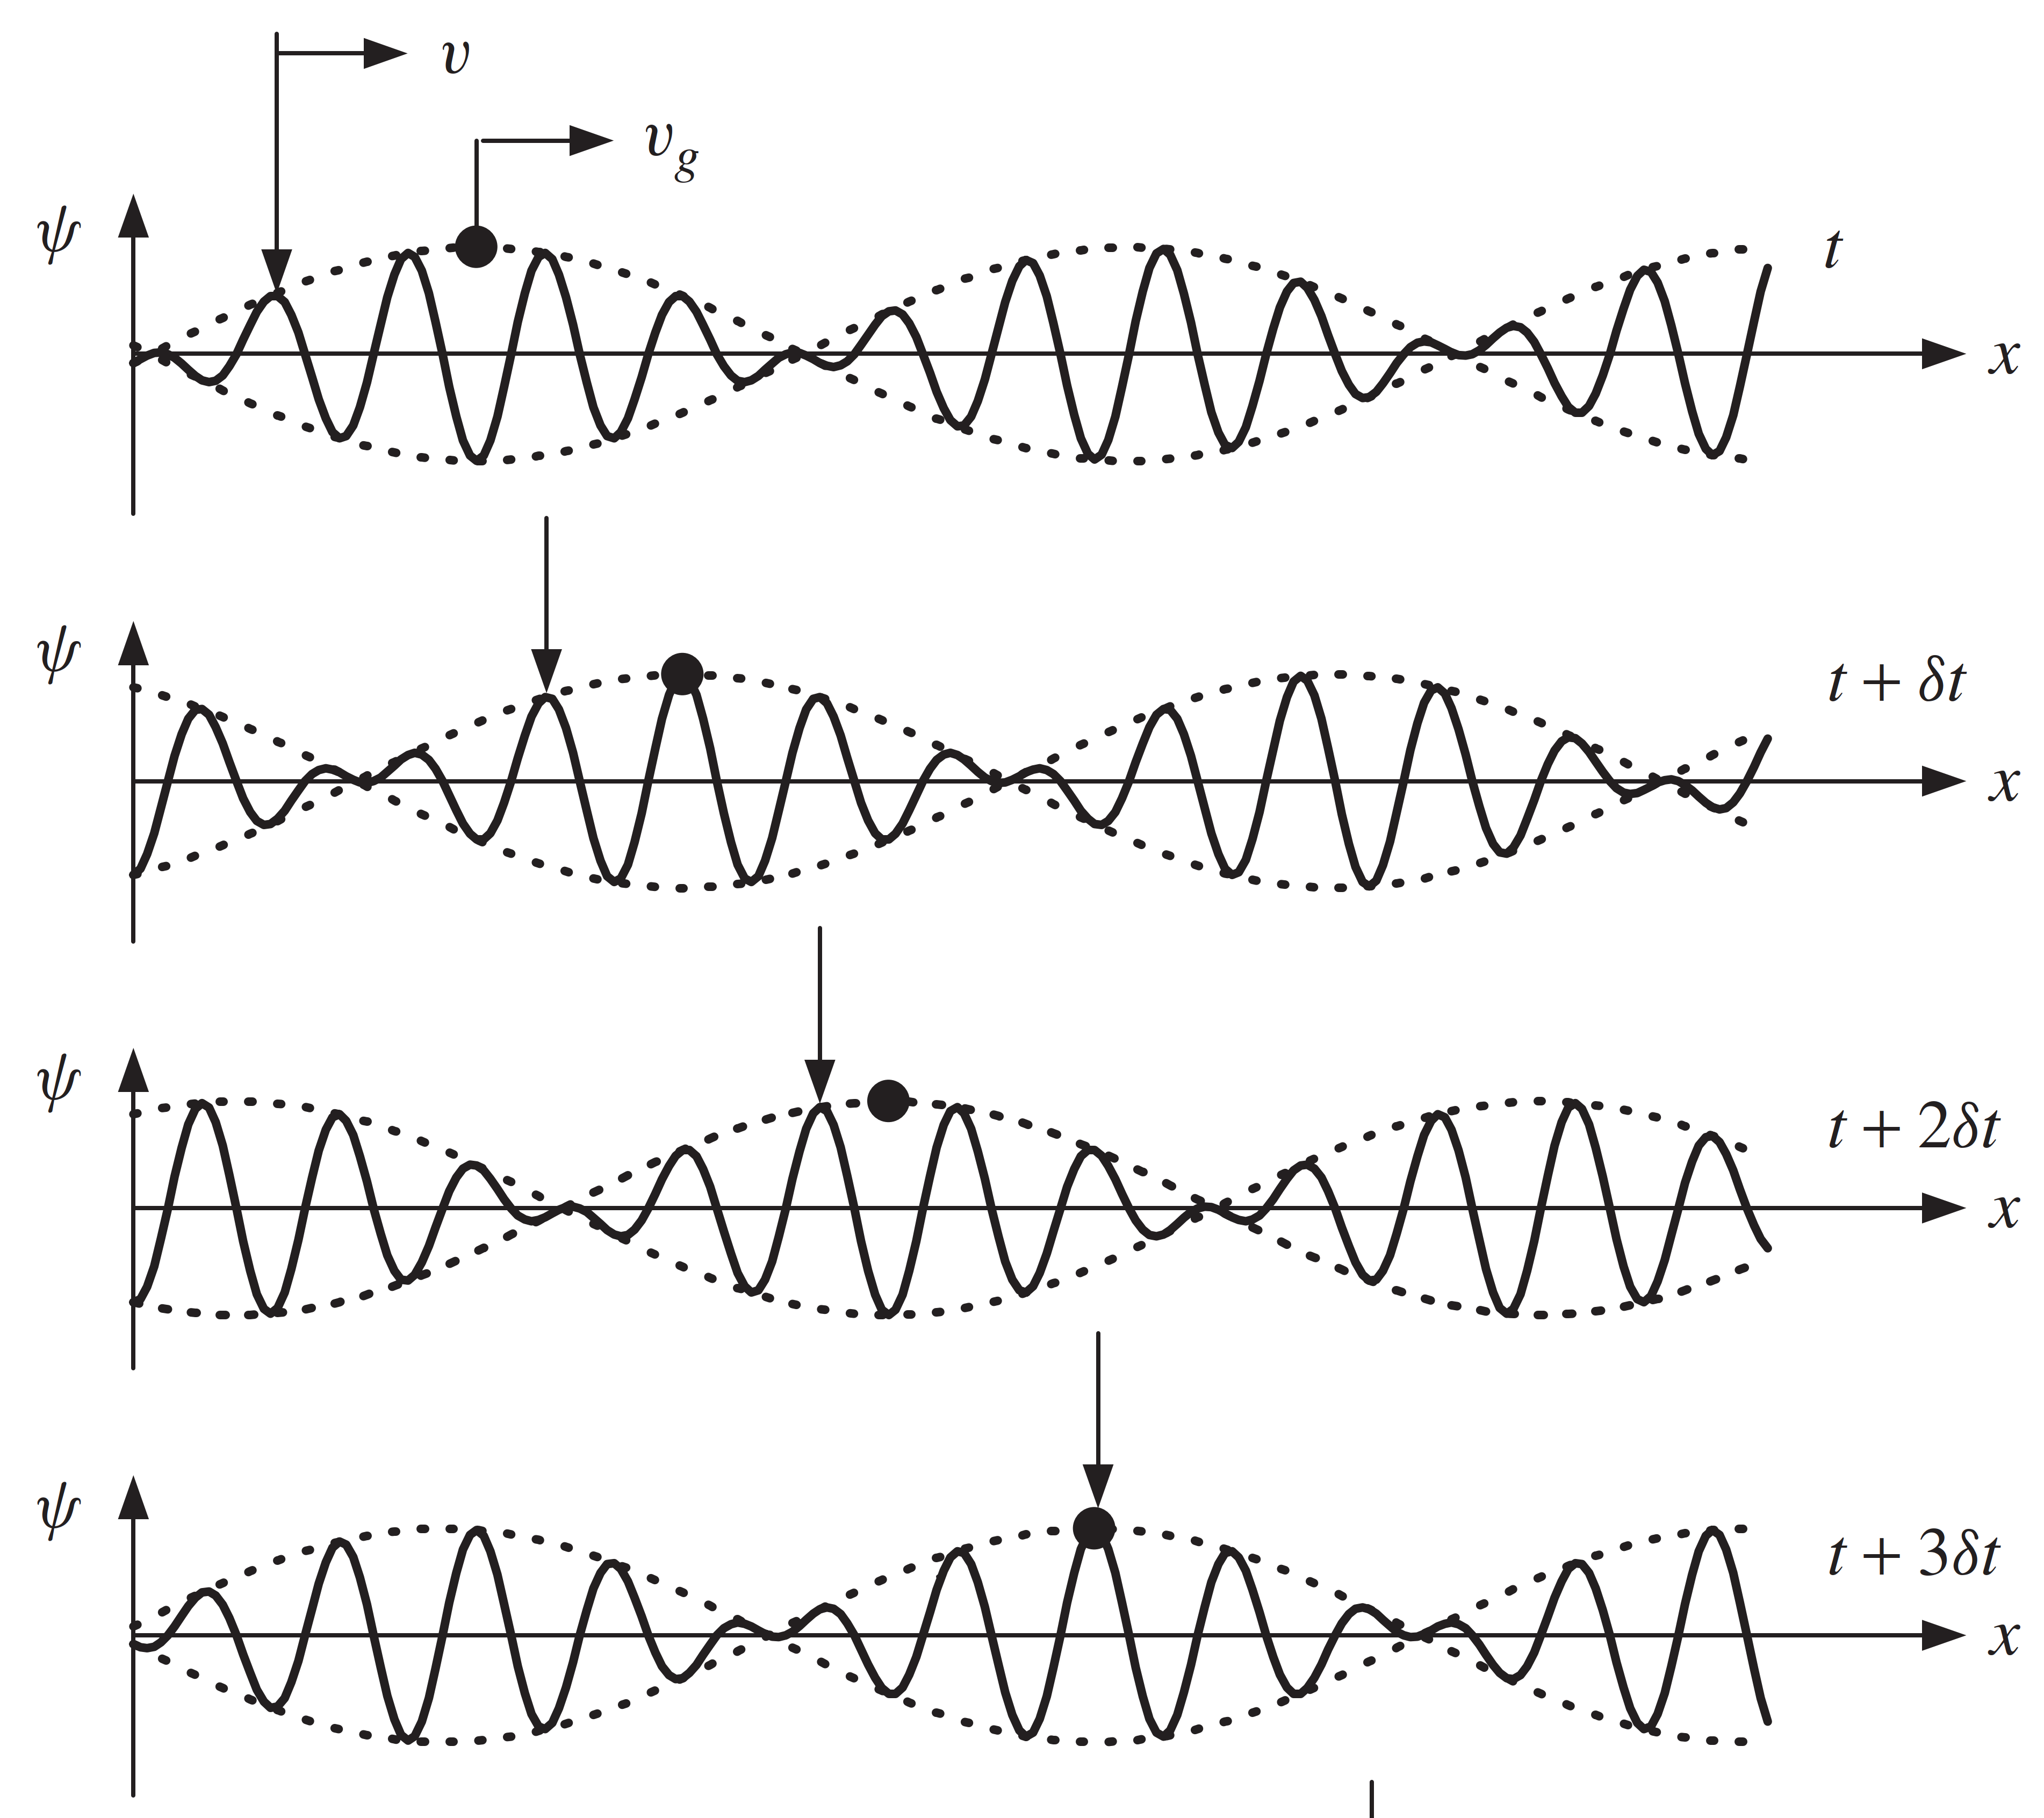
\includegraphics[width=0.65\textwidth]{../Rss/Waves/Dispersion/PhaseGroup.png}
    \caption*{Figure: The propagation of the modulated wave $\psi$ in a dispersive medium}
\end{figure*}

\paragraph{Proof.} From the equation representing modulated wave $\psi$
\begin{equation*}
    \psi=A(x, t) \cos(k_0x - \omega_ot) 
\end{equation*}
we know that 
\begin{equation*}
    k_0x - \omega_ot=\text{Const.}
\end{equation*}
Rearangging this equation, we get the phase velocity at which the wave travels. As for the modulated term
\begin{equation*}
    A=2A cos( \Delta k x- \omega t).
\end{equation*}
we have 
\begin{equation*}
    \Delta k x- \omega t=\text{Const.}
\end{equation*}
Differentiating this equation with respect to $t$, we obtain the velocity at which the envelope travels.

\subsection*{Dispersion Relation}
The relationship between the frequency $\omega$ and the wavenumber $k$ is called the dispersion relation of the medium. The dispersion relation is determined by the physical properties of the medium. In a non-dispersive medium, the velocity of a wave is independent of the wavenumber $k$
\begin{equation*}
    \omega=\text{Const.}\times k
\end{equation*}

The expression for the group velocity, may be rewritten in various different forms
\begin{equation*}
    v_g=\frac{d}{dk}kv=v+k\frac{dv}{dk}=v+k\frac{dv}{d\lambda}\frac{d}{dk} \frac{2\pi}{k}
\end{equation*}
and hence
\begin{equation*}
    v_g=v-\lambda\frac{dv}{d\lambda}
\end{equation*}
Usually $dv/d\lambda$ is positive and so $v_g < v$. This is called normal dispersion (c). Anomalous dispersion occurs when $dv/d\lambda$ is negative so that $v_g > v$ (a). If there is no dispersion, $dv/d\lambda = 0$ and the group and phase velocities are equal (b).
\begin{figure*}
    \centering
    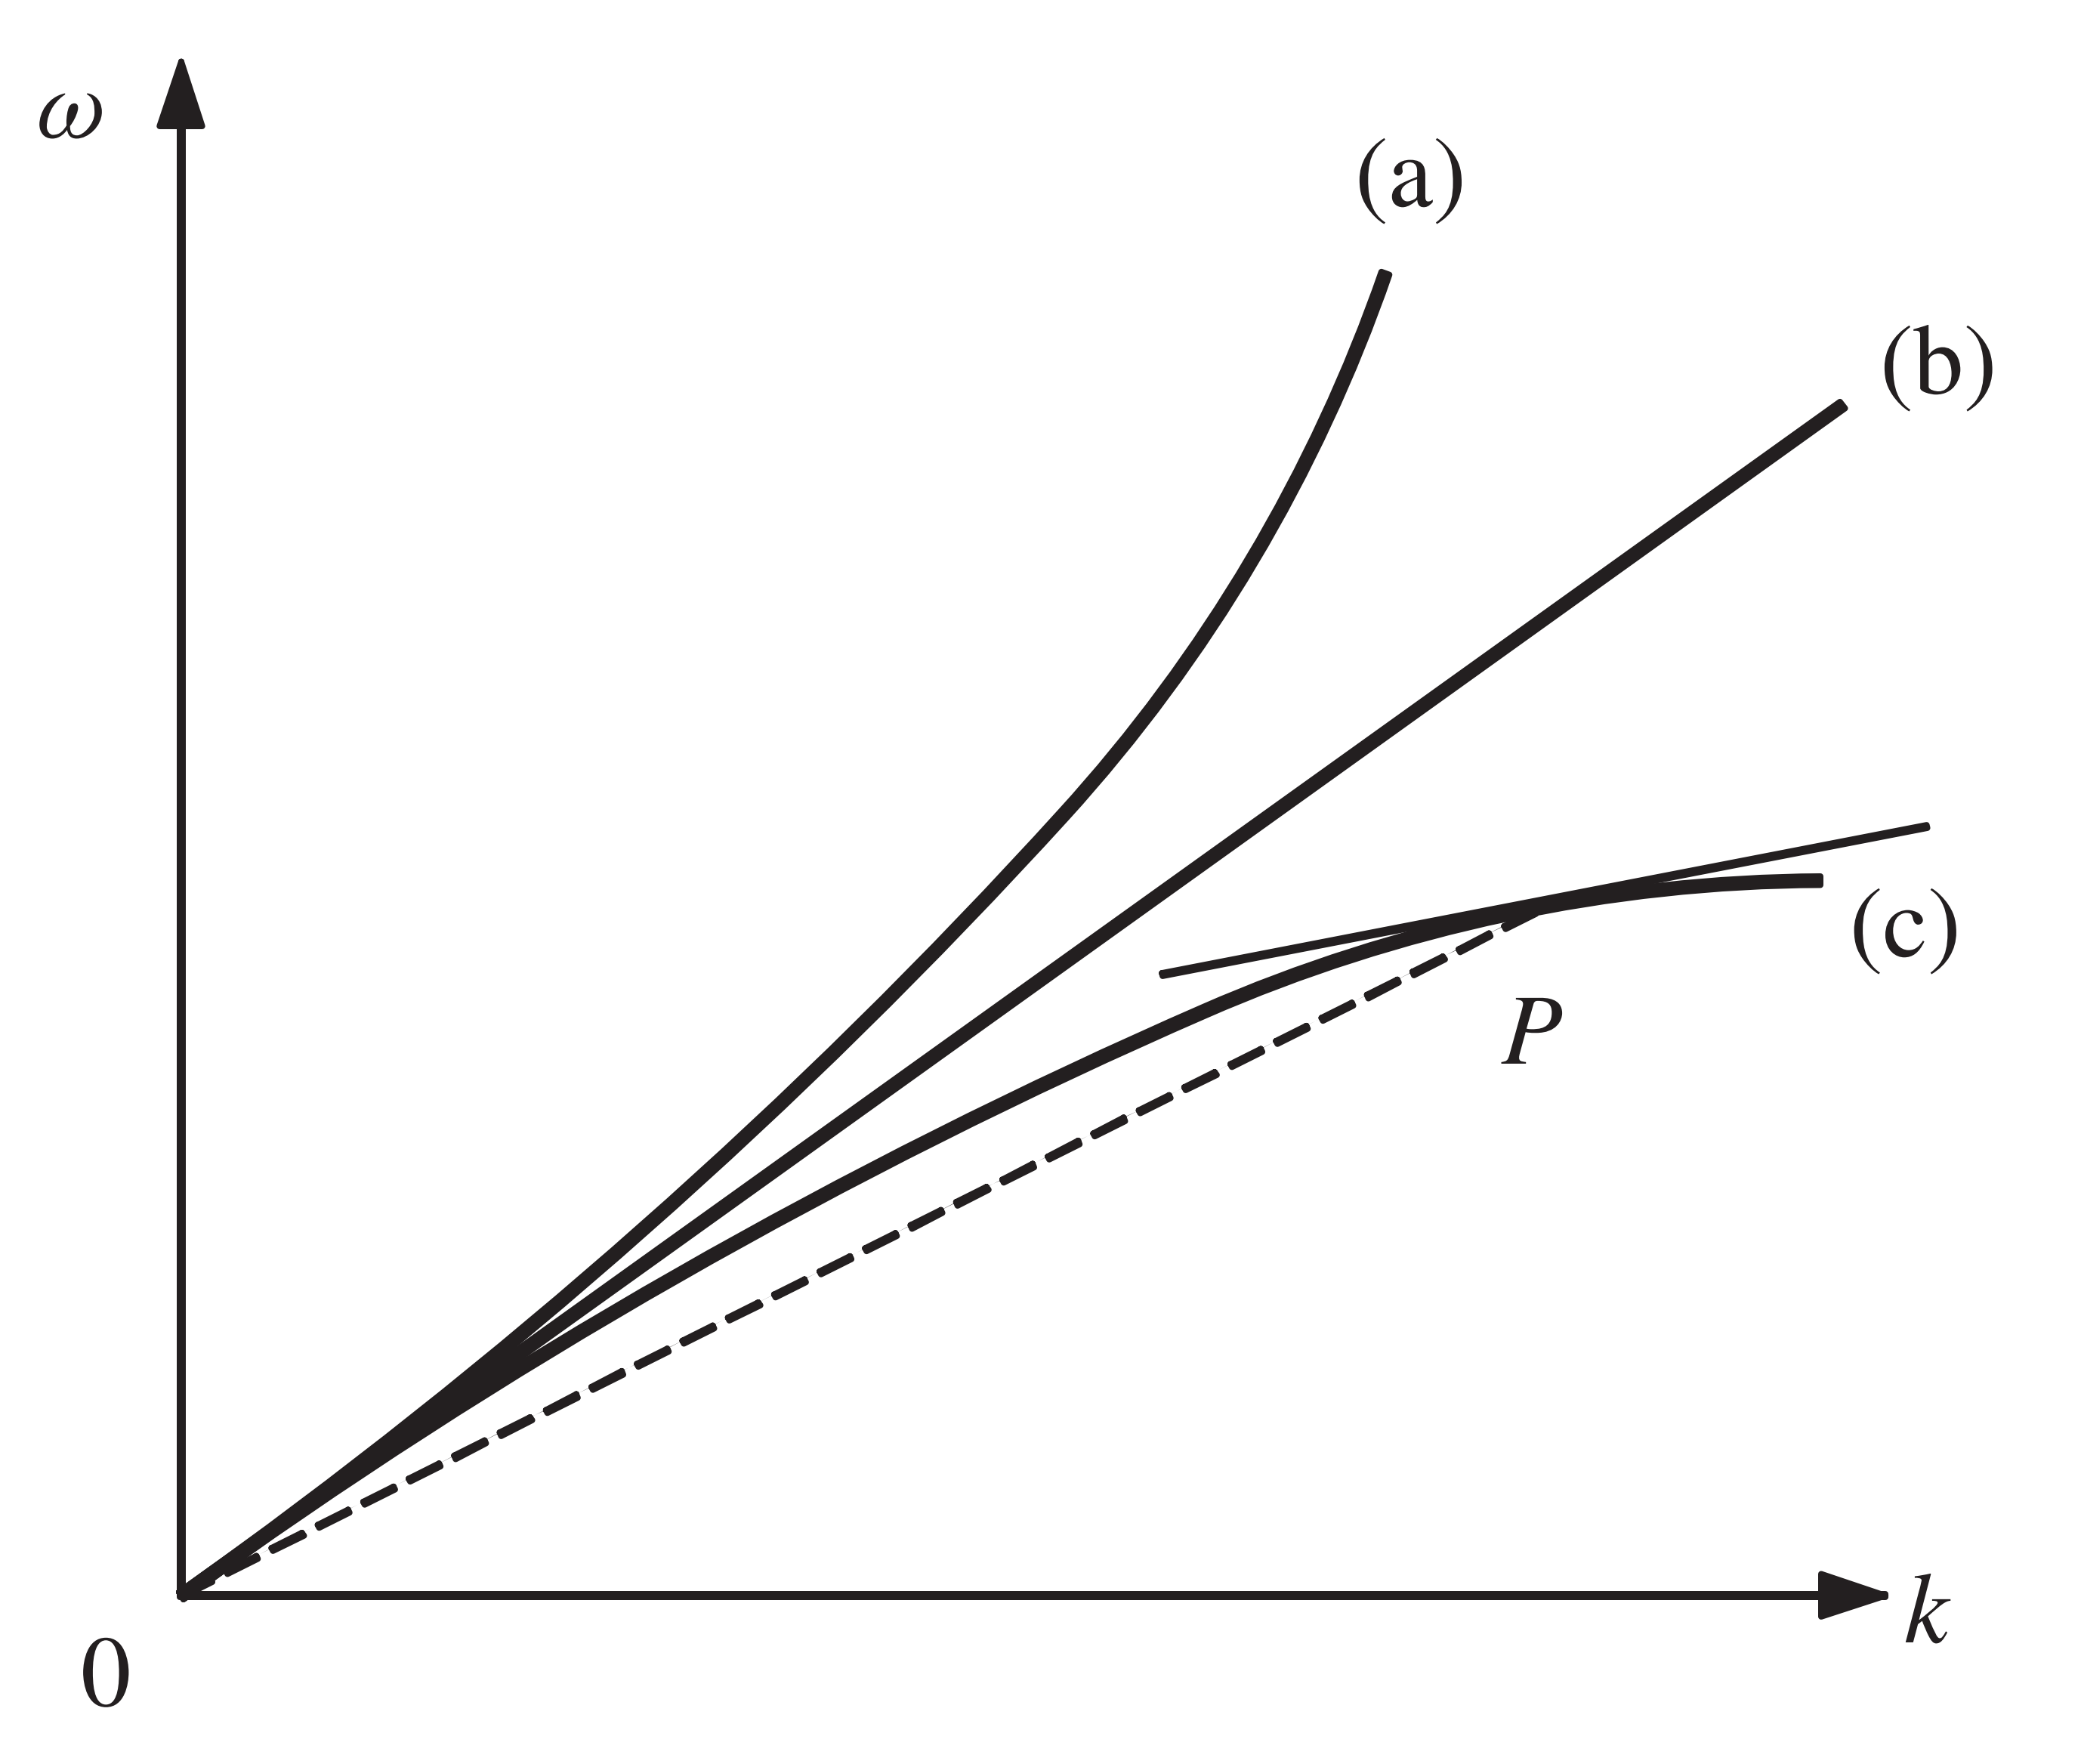
\includegraphics[width=0.6\textwidth]{../Rss/Waves/Dispersion/DispRel.png}
    \caption*{Figure Plots of frequency $\omega$ against wavenumber $k$ for various dispersion relations}
\end{figure*}

\subsubsection*{Electromagnetic Waves.} We can apply these considerations to the propagation of electromagnetic waves. Electromagnetic waves travel with phase velocity 
\begin{equation*}
    v=\frac{c}{\sqrt{1-\dfrac{\omega_0^2}{\omega^2}}}
\end{equation*}
and group velocity
\begin{equation*}
    v_g=c \sqrt{1-\frac{\omega_0^2}{\omega^2}}
\end{equation*}

\paragraph{Proof.} In vacuum, electromagnetic waves propagate with a velocity
\begin{equation*}
    v=\frac{1}{\sqrt{\mu_0\epsilon_0}}
\end{equation*}
while in dielectric 
\begin{equation*}
    v=\frac{1}{\sqrt{\mu\epsilon}}
\end{equation*}
where $\epsilon$ and $\mu$ are the permittivity and permeability of the material, respectively. Now conside the refractive index $n$
\begin{equation*}
    n=\frac{c}{v}=\sqrt{\frac{\mu\epsilon}{\mu_0\epsilon_0}}=\mu_r\epsilon_r
\end{equation*}
where $\mu_r$ and $\epsilon_r$ are the relative permittivity and permeability of the material, respectively. For most materials $\mu_r$ is constant and approximately equal to 1, but $\epsilon
_r$ does vary with frequency. Thus we can write 
\begin{equation*}
    v_g=v-\lambda\frac{d}{d\epsilon_r}\biggl(\frac{c}{\sqrt{\mu_r\epsilon_r}}\biggr) \frac{d\epsilon_r}{d\lambda}=v+\lambda\frac{v}{2\epsilon_r}\frac{d\epsilon_r}{d\lambda}
\end{equation*}The dispersion relation for Electromagnetic waves is 
\begin{align*}
    \omega^2&=\omega_o^2+c^2k^2
\end{align*}
for frequencies greater than $\omega_0$ where $\omega_0$ is a constant called the plasma oscillation frequency. Differentiating this equation gives
\begin{align*}
    2\omega\;d\omega&=2kc^2\;dk\\
    \frac{d\omega}{dk}&=c^2\frac{k}{\omega}
\end{align*}
The phase velocity is the given by 
\begin{align*}
    v&=\frac{\sqrt{\omega_o^2+c^2k^2}}{k}\\
    v&=\frac{c}{ck\biggl(\dfrac{1}{\omega_o^2+c^2k^2}\biggr)^{1/2}}\\
    v&=\frac{c}{\biggl(\dfrac{c^2k^2+\omega_0^2-\omega_0^2}{\omega_o^2+c^2k^2}\biggr)^{1/2}}\\
    v&=\frac{c}{\biggl(1-\dfrac{\omega_0^2}{\omega^2}\biggr)^{1/2}}
\end{align*}
Hence the group velocity is given by 
\begin{equation*}
    v_g=\frac{c^2}{v}=c\sqrt{1-\dfrac{\omega_0^2}{\omega^2}}
\end{equation*}

\subsection*{Wave Packets}
Consider the superposition of a group of monochromatic waves having a set of discrete wavenumbers,
\begin{equation*}
    \psi=\sum_{n}a_n \cos(k_n x - \omega_n t)
\end{equation*}
We need some identities to manipulate the equation above. First we consider
\begin{equation*}
    \sum_{n=0}^{N}e^{inx}
\end{equation*} 
Using complex analysis, we get the useful result
\begin{equation*}
    \sum_{n=0}^{N}\cos nx=\frac{\sin Nx/2}{\sin x/2}\cos\frac{(N-1)}{2}x
\end{equation*}
Then we can write 
\begin{equation*}
    \psi=A(x, t)\cos(k_0 x - \omega_0 t)
\end{equation*}
where 
\begin{equation*}
    A(x, t) = a\frac{\sin[n(x\delta k  -t\delta\omega)/2]}{\sin[(x\delta k  -t\delta\omega)/2]}
\end{equation*}

Suppose now that we have a group of waves that have a continuous distribution of wavenumbers, then the summation is replaced by an integral of the form
\begin{equation*}
    \psi=\int a(k)\cos (kx-\omega t)\;dk
\end{equation*}
Suppose also that the wave amplitude $a(k)$ is given by
\begin{equation*}
    a(k)=\begin{cases}
        \text{if } |k - k_0| \leq   \Delta k/2\\
        \text{if } |k - k_0| >   \Delta k/2
    \end{cases}
\end{equation*}
The superposition of the corresponding group of waves is
\begin{equation*}
    \psi=a\int_{k_0-\Delta k/2}^{k_0+\Delta k/2}\cos (kx-\omega t)\;dk
\end{equation*}
Using Taylor's theorem and assuming that the range of wavenumbers is sufficiently small so that we need to retain only the linear term, we have
\begin{equation*}
    \omega = \omega_o + \alpha(k - k_0)
\end{equation*}
where $\omega_0 = \omega(k_0)$ and $\alpha$ is the derivative term evaluated at $k=k_0$. Hence, substituting for $\omega$ in $(kx - \omega t)$:
\begin{equation*}
    kx - \omega t = k(x - \alpha t) - \beta t
\end{equation*}
where $\beta \equiv \omega_0 - \alpha k_0$. We introduce new variable of integration 
\begin{align*}
    \xi&=k(x - \alpha t) - \beta t\\
    d\xi&= (x - \alpha t)\;dk
\end{align*}
Hence
\begin{equation*}
    \psi=a\int_{\xi_1}^{\xi_2}\frac{\cos \xi}{(x - \alpha t)}\;d\xi
\end{equation*}
with the range of 
\begin{align*}
    \xi_1&=(k_0 -  \Delta k/2)(x - \omega t) - \beta t\\
    \xi_2&=(k_0 +  \Delta k/2)(x - \omega t) - \beta t
\end{align*}
Therefore 
\begin{align*}
    \psi&=\frac{a}{x-\alpha t}\big(\sin\xi_1-\sin\xi_2\big)\\
    &=\frac{2a}{x-\alpha t}\sin \big(\frac{x_1-\xi_2}{2}\big) \cos \big(\frac{x_1+\xi_2}{2}\big)\\
    &=A(x, t) \cos(k_0x - \omega_0 t)
\end{align*}
where
\begin{equation*}
    A(x, t) = a\Delta k\frac{\sin[\Delta k(x-\alpha t)/2]}{\Delta k(x-\alpha t)/2}
\end{equation*}
A familiar result. The sinc first function becomes equal to zero when $x \Delta k/2 =\pm \pi$, giving
\begin{equation*}
    \Delta x\Delta k \approx 2\pi
\end{equation*}
This result is called the bandwidth theorem, which state that the shorter the length of the wave packet, the greater is the range of wavenumbers that is necessary to represent it. Using the relationship $\Delta k=\Delta\omega/v$ and $v=\Delta x/\Delta t$
\begin{equation*}
    \Delta \omega\Delta t\approx2\pi
\end{equation*}
Using $\Delta k=\Delta p/\hbar$
\begin{equation*}
    \Delta p\Delta x\approx h
\end{equation*}
Using $\Delta \omega=\Delta E/\hbar$
\begin{equation*}
    \Delta E\Delta t\approx h
\end{equation*}
\end{document}